\section{Person Isolation}
\label{testing:person isolation}
Figure \ref{fig:depth based cut off} shows the depth based cut off, described in Section \ref{design:person isolation}. As predicted, this cut off is sufficient to eliminate a large proportion of non-person data but does not remove the ring of points at the same depth as the person.\\

\begin{figure}[h]
\begin{center}
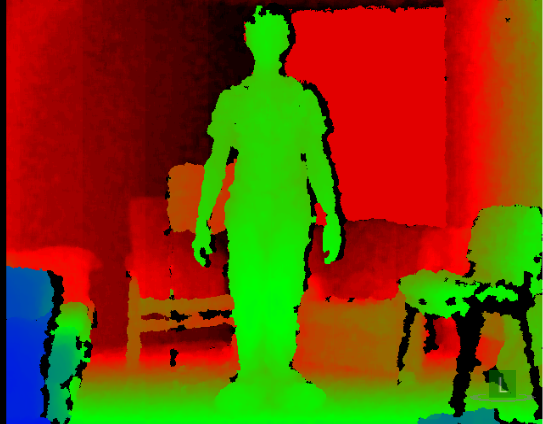
\includegraphics[scale=0.4]{./design/parse1} 
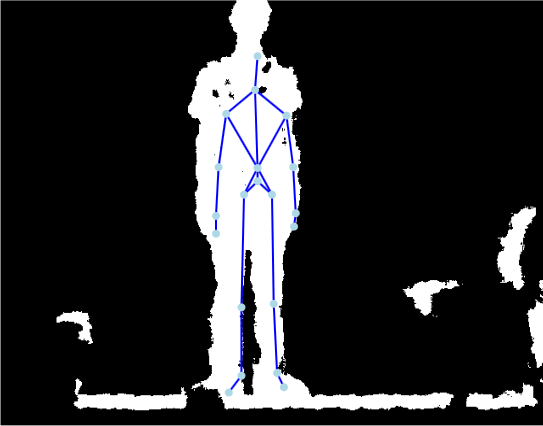
\includegraphics[scale=0.4]{./design/parse2}
\end{center}
\caption{Depth Based Cut Off, before (left) and after (right).}
\label{fig:depth based cut off}
\end{figure} 

Figure \ref{fig:depth and hand based cut off} shows the depth and hand based cut off, described in Section \ref{design:person isolation}. As predicted, the combination of these using depth and hand position is sufficient to isolate a person. The isolated person is coloured from black to white as depth increases away from the camera.\\

\begin{figure}[h]
\begin{center}
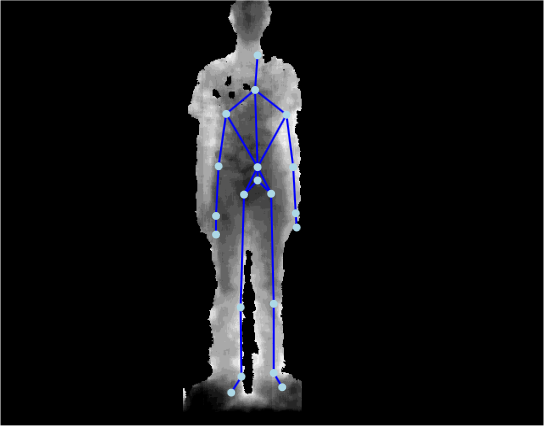
\includegraphics[scale=0.4]{./design/parse3} 
\end{center}
\caption{Depth and Hand Based Cut Off.}
\label{fig:depth and hand based cut off}
\end{figure} 